\documentclass[../distribution_theory_notes.tex]{subfiles}
\begin{document}
\section{Aula 01 - 12/08, 2024}
\subsection{Motivações}
\begin{itemize}
	\item Espaços Vetoriais Topológicos (TVs).
\end{itemize}
\subsection{Espaços Vetoriais Topológicos (TVs)}
Nesse curso, estudaremos propriedades de três espaços de distribuições: \(\mathcal{D'}(\Omega ),\: \mathcal{E'}(\Omega )\) e \(\mathcal{S'}(\mathbb{R}^{n})\), todos definidos
como o dual topológico (que diz respeito não apenas aos funcionais lineares, mas sim àqueles contínuos) de um certo ``Espaço Vetorial Topológico'' cuja topologia não é proveniente de uma norma.
Mais precisamente, poremos:
\begin{align*}
	 & \mathcal{D'}(\Omega )\coloneqq [\mathcal{C}_{c}^{\infty}(\Omega )]'   \\
	 & \mathcal{E'}(\Omega )\coloneqq [\mathcal{C}^{\infty}(\Omega )]'       \\
	 & \mathcal{S'}(\mathbb{R}^{n})\coloneqq [\mathcal{S}(\mathbb{R}^{n})]'.
\end{align*}
Eventualmente, será visto ainda um quarto espaço:
\[
	\mathcal{D'}(\Omega ; \mathcal{S'}(\mathbb{R}^{N})) = [\mathcal{C}_{c}^{\infty}(\Omega ; \mathcal{S}(\mathbb{R}^{N}))]'.
\]

Normalmente, obter uma norma é uma propriedade desejável, afinal permitiria trabalhar com todo o ferramental da análise funcional. Assim, uma pergunta natural que surge é: por que pedimos que os espaços não sejam normados?
Quando analisamos distribuições, queremos algumas propriedades que não são transferidas pelas normas, como a existência de infinitas derivadas e a capacidade de tornar contínuos todos os operadores diferenciais lineares.

Logo, introduziremos nas primeiras aulas os TVS's, que permitirão as construções dos Espaços de Fréchet \(\mathcal{C}^{\infty}(\Omega )\) e \(\mathcal{S}(\mathbb{R}^{n})\), junto ao limite indutivo dos espaços de Fréchet \(\mathcal{C}_{c}^{\infty}(K_{j})\)
dado por
\[
	\mathcal{C}_{c}^{\infty}(\Omega )=\bigcup_{j=1}^{\infty}C_{c}^{\infty}(K_{j}).
\]
Com isso, desejamos obter as propriedades de caráter topológico das distribuições de modo convincente.
\subsection{Uma Breve Introdução aos TVS's}
\begin{def*}
	Seja E um espaço vetorial (poderia ser real, mas será tomado como complexo nessas notas). Dizemos que uma topologia \(\tau \) em E é \textbf{compatível com sua estrutura linear} quando as aplicações
	\begin{align*}
		A: & E\times E\rightarrow E \\
		   & (x, y)\mapsto x+y
	\end{align*}
	e
	\begin{align*}
		M: & \mathbb{C}\times E\rightarrow E      \\
		   & (\lambda , x)\mapsto \lambda \cdot x
	\end{align*}
	são contínuas. Diremos, neste caso, que \(E\times E\) está munido da topologia produto \(\tau \times \tau \) e \(\mathbb{C}\times E\) da topologia produto \(\mathfrak{C}\times \tau \), em que \(\mathfrak{C}\) é a topologial
	usual de \(\mathcal{C}\) que provém do módulo \(|\cdot |.\) Além disso, chamamos \((E, \tau )\) de \textbf{Espaço Vetorial Topológico}. \(\square\)
\end{def*}
Dita por extenso, a definição de um espaço vetorial topológico, doravante TVS (\textit{Topological Vector Spaces}), pede que a soma e a multiplicação por escalares sejam funções contínuas, induzindo
as topologias esperadas em cada espaço-produto. Alguns autores exigem, além da condição de continuidade, que \(\{0\}\) seja um conjunto fechado, o que os tornaria automaticamente espaços Hausdorff.
\begin{example}
	Se \((E, \Vert \cdot  \Vert_{E})\) for um espaço normado, então a topologia que provém da norma é compatível com a estrutura linear de E. Com efeito, como \(E\times E\) é métrico, dada uma sequência
	\((x_{n}, y_{n})\) em \(E\times E\) com \((x_{n}, y_{n})\) convergindo para \((x, y)\), o resultado é que
	\[
		\Vert A(x_{n}, y_{n}) - A(x, y) \Vert_{E} = \Vert (x_{n}+y_{n}) - (x+y) \Vert_{E} \leq \Vert x_{n}-x \Vert_{E} + \Vert y_{n}-y \Vert_{E}\overbracket[0pt]{\longrightarrow}^{n\to \infty}0.
	\]
	Portanto, A é contínua.

	Analogamente, se \((\lambda_{n}, x_{n})\) pertence a \(\mathbb{C}\times E\) e satisfaz ``\((\lambda_{n}, x_{n})\) converge para \((\lambda , x)\)'', então
	\begin{align*}
		\Vert M(\lambda_{n}, x_{n})-M(\lambda , x) \Vert_{E} & =\Vert \lambda_{n}\cdot x_{n} - \lambda \cdot x \Vert                                                                                     \\
		                                                     & = \Vert \lambda_{n}x_{n}-\lambda_{n}x+\lambda_{n}x-\lambda x \Vert_{E}                                                                    \\
		                                                     & \leq |\lambda_{n}|\Vert x_{n}-x \Vert_{E}+|\lambda_{n}-\lambda |\cdot \Vert x \Vert_{E}\overbracket[0pt]{\longrightarrow}^{n\to \infty}0.
	\end{align*}
	Portanto, como antes, M também é contínua.
\end{example}
\begin{example}
	Seja \((E, +, \cdot )\) um espaço vetorial qualquer, \(\tau_{1}=\{\emptyset , E\}\) a \textit{topologia trivial} e \(\tau_{2}=\mathcal{P}(E)\) a \textit{topologia discreta}. Então, \(\tau_{1}\) é compatível com a estrutura linear de E,
	mas \(\tau_{2}\) não é.

	De fato, dado x+y e o aberto E ao qual a soma pertence, tomamos o aberto \(E\times E\), contendo o par ordenado (x, y), tal que tem-se
	\[
		A(E\times E)=E \Rightarrow A^{-1}(\emptyset )=\emptyset \quad\&\quad A^{-1}(E)=E\times E.
	\]
	Para a multiplicação por escalar, o processo é análogo.

	Por outro lado, embora A seja contínua com respeito a \(\tau_{2}\), M não é, pois se \(\lambda \) é um número complexo e x é não-nulo, não existe \(\delta >0\) tal que
	\[
		M(B(\lambda; \delta )\times \{x\})\subseteq \{\lambda x\}=U\in \mathcal{P}(E).
	\]
\end{example}
\begin{example}
	Um exemplo menos trivial é o seguinte: sejam \(0 < p < 1\) e considere o espaço \((L^{p}(I), \Vert \cdot \Vert_{p})\), em que
	\[
		L^{p}(I) = \biggl\{f:I\rightarrow \mathbb{C}: f \text{ é mensurável e } \int_{I}^{}|f(t)|^{p}dt < \infty\biggr\},
	\]
	e a norma é
	\[
		\Vert f \Vert_{p}\coloneqq \biggl(\int_{I}^{}|f(t)|^{p}dt\biggr)^{\frac{1}{p}}.
	\]
	Sabemos que \(\Vert \cdot  \Vert_{p}\) não define uma norma em \(L^{p}\). Porém,
	\[
		d(f, g)\coloneqq \Vert f-g \Vert_{p}^{p} = \int_{I}^{}|f(t)-g(t)|^{p}dt
	\]
	é uma distância que induz uma topologia em \(L^{p}\), ou seja, ele é um TVS.

	Realmente, pois, utilizando que \(0 < p < 1\), obtemos
	\[
		(a+b)^{p}\leq a^{p}+b^{p},\quad \forall a, b\geq 0,
	\]
	donde decorrem duas coisas: a desigualdade triangular para a distância entre funções como foi definida E o fecho de \(L^{p}\) para a soma.

	Com esses dois fora do caminho, podemos analisar a estrutura topológica necessária para confirmar que ele é de fato um TVS - em outras palavras, vamos conferir a continuidade da soma e multiplicação por escalar.
	Precisamos, para isso, entender o que seria exatamente a continuidade nesse contexto; como temos uma estrutura métrica no espaço \(L^{p}\), segue que podemos utilizar bolas centradas em algum ponto como os abertos (na verdade,
	vale lembrar que os abertos na topologia induzida pela métrica são uniões de bolas abertas, mas enfim). Sendo assim, considerando um centro em \(f_{0}+g_{0}\) para o domínio \(L^{p}(I)\times L^{p}(I)\) da soma
	e duas bolas no contradomínio dela, \(L^{p}\), uma centrada em \(f_{0}\) e outra em \(g_{0}\), a prova seguirá a partir da seguinte desigualdade métrica:
	\begin{align*}
		d(f+g, f_{0}+g_{0}) & = \int_{I}^{}|(f-f_{0})+(g-g_{0})|^{p} dt   \\
		                    & \leq \int_{I}^{}[|f-f_{0}|+|g-g_{0}|]^{p}dt \\
		                    & \leq d(f, f_{0}) + d(g, g_{0}).
	\end{align*}
	Por outro lado, quando \((\lambda, f)\) converge para \((\lambda_{0}, f_{0})\) em \(L^{p}\), segue que
	\begin{align*}
		d(\lambda f, \lambda_{0}f_{0}) & = \int_{I}^{}|\lambda f - \lambda_{0}f_{0}|^{p}dt                                                                                                          \\
		                               & = \int_{I}^{}|\lambda(f-f_{0}) + (\lambda-\lambda_{0})f_{0}|^{p}dt                                                                                         \\
		                               & \leq |\lambda|^{p}d(f, f_{0}) + |\lambda -\lambda_{0}|^{p}\Vert f_{0} \Vert_{p}^{p}\overbracket[0pt]{\longrightarrow}^{(\lambda, f)\to (\lambda, f_{0})}0.
	\end{align*}
	Portanto, tanto a soma quanto a multiplicação por escalar são contínuas, assim concluindo a prova de que \(L^{p}\) é um TVS.
\end{example}

Para conseguirmos conversar sobre TVS de maneira mais fluída, é importante dedicar um tempo ao estabelecimento de uma linguagem comum que possamos entender ao longo do tratado. Sejam \((E, +, \cdot )\) um espaço vetorial, A e B seus subconjuntos, e \(\lambda \) um número complexo. Escreve-se:
\begin{itemize}
	\item[i)] \( A+B\coloneqq \{x + y:x\in A,\: y\in B\}\);
	\item[ii)] se a pertence ao conjunto E, \(a+B\coloneqq \{a + y:y\in B\}\);
	\item[iii)] \(\lambda A \coloneqq \{\lambda \cdot x: x\in A\}\) e, mais geralmente, se \(\Lambda\) é um subconjunto dos números complexos, \(\Lambda A \coloneqq \{\lambda \cdot x: \lambda \in \Lambda,\:x\in A \}\)
	\item[iv)] A é \textbf{convexo} quando
	      \[
		      tA + (1-t)A\subseteq A,\quad \forall t\in [0, 1]
	      \]
	\item[v)] B é \textbf{equilibrado/balanceado} quando
	      \[
		      \lambda B \subseteq B,\quad \forall \lambda \in \mathbb{C}:\:|\lambda |\leq 1
	      \]
	      Dito de forma equivalente, ele será equilibrado quando o conjunto dos produtos de B por uma bola unitária fechada continua dentro de B:
	      \[
		      \overline{B}(0;1)\cdot B\subseteq B.
	      \]
	\item[vi)] B é \textbf{absorvente} quando, dado x em E, existe um r positivo \textit{dependendo de x}, tal que \(\lambda x\) cai pra dentro de B para todo escalar menor que r em módulo:
	      \[
		      \forall x\in E,\: \exists r=r(x)>0: \:\lambda x\in B,\quad \forall \lambda \in \mathbb{C}:\:|\lambda |\leq r.
	      \]
	      Há ainda uma outra definição, com foco no conjunto ao invés do elemento:
	      \[
		      \exists s > 0:\: x\in tB,\quad \forall t \geq s.
	      \]
\end{itemize}
Vejamos algumas imagens para ilustrar!
\begin{figure}[H]
	\begin{center}
		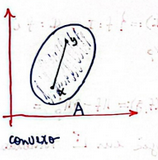
\includegraphics[height=0.25\textheight, width=0.25\textwidth, keepaspectratio]{./Images/convex.png}
	\end{center}
	\caption{Conjunto Convexo.}
	\label{conv1}
\end{figure}

\begin{figure}[H]
	\begin{center}
		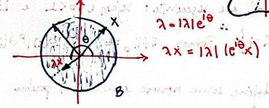
\includegraphics[height=0.25\textheight, width=0.25\textwidth, keepaspectratio]{./Images/balanced.png}
	\end{center}
	\caption{Conjunto Balanceado que não seja um estrela sem pontas.}
	\label{bal1}
\end{figure}

\begin{figure}[H]
	\begin{center}
		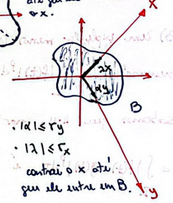
\includegraphics[height=0.25\textheight, width=0.25\textwidth, keepaspectratio]{./Images/absorbing.png}
	\end{center}
	\caption{Conjunto absorvente que segue a definição dada, com a ideia de contrair x até ele entrar em B.}
	\label{abs1}
\end{figure}


\begin{figure}[H]
	\begin{center}
		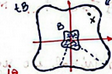
\includegraphics[height=0.25\textheight, width=0.25\textwidth, keepaspectratio]{./Images/absorbing_rudin.png}
	\end{center}
	\caption{Conjunto absorvente com uma ideia que segue o Rudin: ao invés de contrair x até ele entrar em B, dilata-se B até que ele absorva o x.}
	\label{abs2}
\end{figure}

Note que, se B é absorvente ou equilibrado, ele necessariamente contém o 0, mas um convexo não precisa disso. Além disso, não é verdade que
\[
	2A = A + A,
\]
mas sempre temos
\[
	2A \subseteq A + A.
\]
Em particular, a outra inclusão também ocorre quando A é convexo.

Podemos expressar a continuidade de A e de M em (0, 0) de um TVS em termos das notações de operações ``entre conjuntos'' (i a iii). Com efeito, se U é uma vizinhança do 0 em E, então a pré-imagem de U pela adição contém um aberto Z de \(E\times E\) que contém o (0, 0);
por sua vez, o (0, 0) deve estar contido em um ``retângulo'' formado por abertos da forma
\[
	W\times W'\ni (0, 0).
\]
Colocando, então, \(V\coloneqq W\cap W'\), o qual contém o 0 (já que pertence a ambos), segue que V é um aberto de E e que
\[
	V\times V\subseteq A^{-1}(U)\Rightarrow V + V = A(V)\subseteq A(A^{-1}(U))\subseteq U.
\]
Em suma, se U é um aberto de E que contém o 0, existe um aberto V, também contendo o 0, cuja soma consigo mesmo é um subconjunto de U.
\begin{exr}
	Escreva a mesma coisa, mas com relação a M.
\end{exr}

Em seguida, veremos algumas propriedades dos TVS quando sofrem uma transformação rígida\footnote{Ou seja, que preservam distâncias entre pontos. Exemplos clássicos seriam translação, dilatação e rotação.}

\begin{lemma*}
	Seja \((E, \tau )\) um TVS. Dados \(\lambda_{0}\) um número complexo não nulo e elementos a, \(x_{0}\) de E quaisquer, consideremos as aplicações
	\begin{itemize}
		\item[1)] \(T_{a}:E\rightarrow E,\: T_{a}(x) = x + a\);
		\item[2)] \(M_{\lambda_{0}}:E\rightarrow E,\: M_{\lambda_{0}}(x)\coloneqq \lambda_{0}\cdot x\);
		\item[3)] \(m_{x_{0}}:\mathbb{C}\rightarrow E,\: m_{x_{0}}(\lambda)\coloneqq \lambda \cdot x_{0}\).
	\end{itemize}
	Então, \(T_{a},\: M_{\lambda_{0}} \) são homeomorfismos e \(m_{x_{0}}\) é contínua.
\end{lemma*}
Antes de prosseguir à prova, vale comentar que, por conta de \(T_{a}\) - translação de um ponto x por a unidades - ser um homeomorfismo,
diz-se que a topologia de um TVS é \textit{invariante por translação}, o que significa que, topologicamente,
ela se parece da mesma forma ao redor de qualquer ponto, não importa qual seja.
\begin{proof*}
	De outros cursos, sabe-se que \(T_{a}\) e \(M_{\lambda_{0}}\) são bijeções cujas inversas caracterizam-se por
	\[
		T_{-a} \quad\&\quad M_{\lambda_{0}^{-1}}.
	\]
	Por outro lado, considerando as inclusões contínuas (devido à definição da topologia produto)
	\begin{align*}
		 & i_{a}:E\rightarrow E\times E,\: i_{a}(x)\coloneqq (a, x);                                   \\
		 & j_{\lambda_{0}}:E\rightarrow E\times E,\: j_{\lambda_{0}}(x)\coloneqq (\lambda_{0}, x);     \\
		 & k_{x_{0}}:\mathbb{C}\rightarrow E\times E,\: k_{x_{0}}(\lambda )\coloneqq (\lambda, x_{0}). \\
	\end{align*}
	Assim, basta ver que
	\[
		T_{a} = A\circ i_{a},\quad M_{\lambda_{0} = M\circ j_{\lambda_{0}} }\quad\&\quad m_{x_{0}} = M\circ K_{x_{0}},
	\]
	e o lema está provado. \qedsymbol
\end{proof*}
\begin{crl*}
	A adição é uma aplicação aberta (leva abertos em abertos).
\end{crl*}
\begin{proof*}
	Com efeito, se \(U\times V\) é um aberto básico de \(E\times E\), então
	\[
		A(U\times V) = U + V = \bigcup_{a\in U}^{}(a+V) = \bigcup_{a\in U}^{}T_{a}(V).
	\]
	Portanto, como \(T_{a}\) é aberta (por ser homeomorfismo), a última igualdade é nada mais, nada menos, que uma união de abertos de E. \qedsymbol
\end{proof*}
\begin{theorem*}
	Se \(\mathcal{B}\) é um \hyperlink{sistema_fundamental_vizinhas}{\textit{sistema fundamental de vizinhanças}} da origem em um TVS e a é um elemento qualquer de E, então
	\[
		\mathcal{B}_{a}\coloneqq \{a + V:\:V\in \mathcal{B}\}
	\]
	é um \hyperlink{sistema_fundamental_vizinhas}{\textit{sistema fundamental de vizinhanças}} do ponto a.
\end{theorem*}
\begin{proof*}
	A prova segue de imediato, já que, se U é um aberto de E tal que a pertence a ele, então
	\[
		T_{-a}(U) = U-a\in\tau_{E},
	\]
	sendo que
	\[
		0 = a - a = T_{-a}(a) \Rightarrow 0\in U-a.
	\]
	Logo, existe B em \(\mathcal{B}\) que contém o 0 e é subconjunto de \(U-a\)

	Portanto, \(B+a\) é um subconjunto de U e \(B+a\) pertence a \(\mathcal{B}\). \qedsymbol
\end{proof*}
\begin{theorem*}
	Todo aberto B de E que contém a origem é absorvente (em outras palavras, toda vizinhança da origem é absorvente).
\end{theorem*}
\begin{proof*}
	Com efeito, dado x em E e utilizando a continuidade de \(m_{x}:\mathbb{C}\rightarrow E\), vale que \(m_{x}^{-1}(B)\) é um aberto de \(\mathbb{C}\) que contém a origem, já que
	\[
		m_{x}(0)=0 \cdot x = 0\in B.
	\]
	Logo, existe um \(r_{x}\) positivo tal que
	\[
		B_{\mathbb{C}}(0; r_{x}) \subseteq m_{x}^{-1}(B),
	\]
	que se traduz na existência desse tal \(r_{x}\) que satisfaz
	\[
		|\lambda |\leq r_{x}\Rightarrow \lambda x \in B.
	\]
	Portanto, B é absorvente. \qedsymbol
\end{proof*}
\end{document}
